\documentclass[tikz,border=5pt]{standalone}
\usepackage{amsmath,amssymb,amsthm}
\usetikzlibrary{decorations.pathreplacing}

\begin{document}
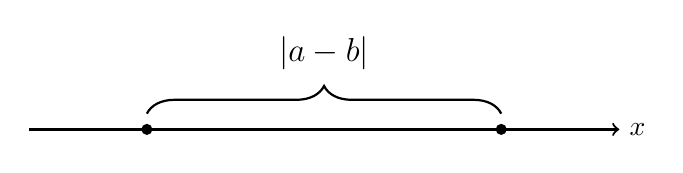
\begin{tikzpicture}[x=1cm, y=1cm]

  % 1. The number line (axis)
  \draw[->, thick] (-4.5,0) -- (3,0) node[right] {\(x\)};

  % 2. The actual points (black dots)
  \fill (-3,0) circle (2pt);
  \fill (1.5,0) circle (2pt);

  % 3. The big curly brace
  % mirror makes it point upwards, amplitude is how tall it is
  \draw[decorate, decoration={brace, amplitude=10pt}, thick]
    (-3, 0.2) -- (1.5, 0.2)
    node[midway, above=12pt] {\large $\lvert a - b \rvert$};

\end{tikzpicture}
\end{document}